% =====================================================================
% Snippet: gaussian-curve.tex
% =====================================================================
% USAGE: Normal distribution curve with optional shaded region
% (1σ / 2σ / critical region for hypothesis test).
% Used in: probability theory / hypothesis test / confidence interval.
%
% Copy %% COPY-START / END, replace:
%   - mu: mean (default 0)
%   - sigma: std dev (default 1)
%   - x_min, x_max: x-axis range
%   - shade_left, shade_right: shaded region boundaries (in x units)
%   - chart_W, chart_H: plot area
% =====================================================================

\documentclass[tikz,border=10pt]{standalone}
\usepackage{xcolor,tikz}
\usetikzlibrary{positioning,calc}

\definecolor{acaBlueLine}{HTML}{3060A8}
\definecolor{acaBlueFill}{HTML}{DCE6F4}
\definecolor{acaOrangeLine}{HTML}{D06020}
\definecolor{acaOrangeFill}{HTML}{F9E0D0}
\definecolor{acaGreyLine}{HTML}{606060}

\begin{document}
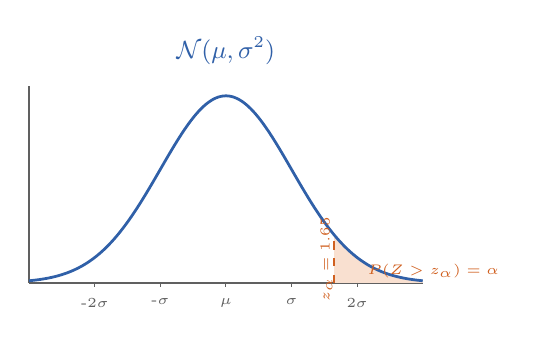
\begin{tikzpicture}

%% COPY-START =========================================================

\def\xO{0}
\def\yO{0}
\def\chartW{5.0}
\def\chartH{2.5}
\def\xMin{-3}
\def\xMax{3}
\def\yMax{0.42}   % peak of N(0,1) is 1/sqrt(2π) ≈ 0.4

% --- AXES ---
\draw[acaGreyLine, line width=0.5pt]
  (\xO, \yO) -- (\xO + \chartW, \yO);    % x-axis
\draw[acaGreyLine, line width=0.5pt]
  (\xO, \yO) -- (\xO, \yO + \chartH);    % y-axis

% Helper: map data x to canvas x
\pgfmathsetmacro\xScale{\chartW / (\xMax - \xMin)}
\pgfmathsetmacro\yScale{\chartH / \yMax}

% --- SHADED REGION (e.g., critical region x > 1.96) ---
\def\shadeStart{1.65}
\def\shadeEnd{3.0}
\fill[acaOrangeFill]
  plot[domain=\shadeStart:\shadeEnd, samples=40]
    ({\xO + (\x - \xMin) * \xScale},
     {\yO + (1/sqrt(2*pi)) * exp(-\x*\x/2) * \yScale})
  -- ({\xO + (\shadeEnd - \xMin) * \xScale}, \yO)
  -- ({\xO + (\shadeStart - \xMin) * \xScale}, \yO)
  -- cycle;

% --- GAUSSIAN CURVE: y = (1/√2π) · exp(-x²/2) ---
\draw[acaBlueLine, line width=1.0pt]
  plot[domain=\xMin:\xMax, samples=80, smooth]
    ({\xO + (\x - \xMin) * \xScale},
     {\yO + (1/sqrt(2*pi)) * exp(-\x*\x/2) * \yScale});

% --- X-AXIS TICKS at -2σ, -σ, 0, σ, 2σ ---
\foreach \xv/\lab in {-2/-2$\sigma$, -1/-$\sigma$, 0/$\mu$, 1/$\sigma$, 2/2$\sigma$} {
  \pgfmathsetmacro\xpos{\xO + (\xv - \xMin) * \xScale}
  \draw[acaGreyLine, line width=0.3pt] (\xpos, \yO) -- (\xpos, \yO - 0.05);
  \node[anchor=north, font=\tiny, color=acaGreyLine]
    at (\xpos, \yO - 0.08) {\lab};
}

% --- CRITICAL VALUE ANNOTATION ---
\pgfmathsetmacro\zCritX{\xO + (1.65 - \xMin) * \xScale}
\draw[acaOrangeLine, dashed, line width=0.5pt]
  (\zCritX, \yO) -- (\zCritX, \yO + 0.6);
\node[anchor=south, font=\tiny, color=acaOrangeLine, rotate=90]
  at (\zCritX + 0.1, \yO + 0.3) {$z_{\alpha} = 1.65$};

% --- LABELS ---
\node[anchor=south, font=\small\bfseries, color=acaBlueLine]
  at (\xO + \chartW/2, \yO + \chartH + 0.15)
  {$\mathcal{N}(\mu, \sigma^2)$};
\node[anchor=west, font=\tiny, color=acaOrangeLine]
  at (\zCritX + 0.3, \yO + 0.15)
  {$P(Z > z_\alpha) = \alpha$};

%% COPY-END ===========================================================

\end{tikzpicture}
\end{document}
